\documentclass[windows,csize4]{BHCexam}
%\documentclass[windows,csize4,answers]{BHCexam}

\usepackage{multicol} % 分栏
\usepackage{polynom} % 多项式除法
\pagestyle{fancy}
\fancyfoot[C]{\kaishu \small 第 \thepage 页 共 \pageref{lastpage} 页}
%\fancyhead[L]{\includegraphics[width=2cm]{qrcode.png}}
\title{因式分解 - 对称式和轮换式}
%\subtitle{数学文科试卷}
%\notice{满分150分, 120分钟完成, \\	允许使用计算器,答案一律写在答题纸上.}
%\author{Gavin Chen}
%\date{\today}
\usepackage{enumerate} % 编号
\usepackage{cases}

\begin{document}

\maketitle

\begin{groups}
    \group{前言}{}
    物理学是一门怎样的学科。
    \begin{itemize}
        \item 物理——万物之理。
        \item 实践是一切知识的试金石;实验是科学“真理”的唯一鉴定者。
        \item 物理学中的分工:理论物理学家想象、推演和猜测新的定律;实验物理学家进行实验、想象、推演和猜测。
    \end{itemize}
    
    \group{长度的测量}{}
    关于测量,眼见不一定为实,所以需要测量。
    图 \ref{fig:fig_1_1}中$AB$,$CD$哪个线段更长?
    \begin{figure}[htb]
        \centering
        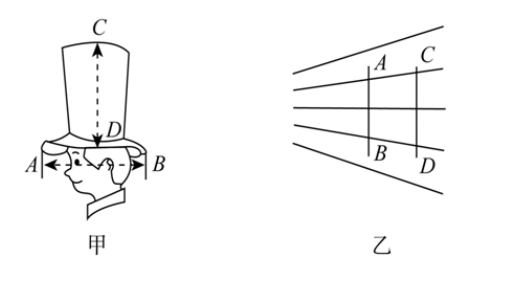
\includegraphics [scale=0.75,trim=0 0 0 0]{./image/fig_1_1.PNG}
        \caption{$AB$,$CD$哪个线段更长} 
        \label{fig:fig_1_1}
    \end{figure}

    图 \ref{fig:fig_1_2}中$AB$,$CD$是否平行?$EFGH$是否是正方形?
    \begin{figure}[htb]
        \centering
        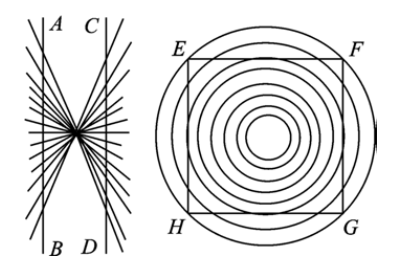
\includegraphics [scale=0.75,trim=0 0 0 0]{./image/fig_1_2.PNG}
        \caption{$AB$,$CD$是否平行?$EFGH$是否是正方形} 
        \label{fig:fig_1_2}
    \end{figure}




    

\end{groups}





\label{lastpage}
\end{document}